\section{Problem}
\label{section:problem}
%%%%%%%%%%%%%%%%%% NOTATION %%%%%%%%%%%%%%%%%%%%%%%%%%
\newcommand{\varTime}[2]{\phi}
\newcommand{\setTime}[2]{\Phi}
\newcommand{\varAtomicTask}[2]{\varSymbol{tp}{#1}{#2}}
\newcommand{\varCompositeTask}[2]{\varSymbolHat{tp}{#1}{#2}}
\newcommand{\varAgent}[2]{g_{#1}^{#2}}
\newcommand{\setAgents}[2]{G_{#1}^{#2}}
\newcommand{\varIdleAgent}[2]{\varAgent{i}{}}  
\newcommand{\varSleepAgent}[2]{\varAgent{s}{}}  
\newcommand{\varChildAgent}[2]{\varAgent{c}{}}    
\newcommand{\varParentAgent}[2]{\varAgent{p}{}}

\newcommand{\varOrchestrationEnergy}[2]{OE}
\newcommand{\varTransmissionEnergy}[2]{TE}
\newcommand{\varReceiverEnergy}[2]{RE}
\newcommand{\varIdleEnergy}[2]{IE}
\newcommand{\varSleepEnergy}[2]{SE}
\newcommand{\varSystemEnergyConsumption}[2]{sec_{\setTime{}{}}}
\newcommand{\varTaskEnergy}[2]{tec_{\varCompositeTask{}{}}}
\newcommand{\setTaskEnergy}[2]{TEC_{\varCompositeTask{}{}}}
\newcommand{\varSystemEnergyVariability}[2]{sev_{\varTime{}{}}}

\newcommand{\varAgentEnergyAvailable}[2]{aea_{\varAgent{}{},\varTime{}{}}}
\newcommand{\functionAgentEnergyTotal}[2]{
	\functionSignature{aet_{\varAgent{}{},\varTime{}{}}}
	{\varAgent{#1}{#2}}
}

\newcommand{\setAgentEnergyAvailable}[2]{\mathrm{AEA}_{\varAgent{}{},\varTime{}{}}}
\newcommand{\functionSystemEnergyAvailable}[2]{
	\functionSignature{sea_{\varTime{}{}}}{\setAgents{}{}}
}

\newcommand{\functionProbabilityInit}[2]{
	\functionSignature{pinit}{\varAgent{}{}}
}
\newcommand{\functionProbabilityRand}[2]{
	\functionSignature{prand}{\varAgent{}{}}
}
\newcommand{\functionProbabilityWear}[2]{
	\functionSignature{pwear}{\varAgent{}{}}
}
\newcommand{\functionProbabilityFail}[2]{
	\functionSignature{pfail}{\varAgent{}{}}
}
\newcommand{\varConstantInit}[2]{{C}{INIT}^{#2}}
\newcommand{\varConstantRand}[2]{{C}{RAND}^{#2}}
\newcommand{\varConstantWear}[2]{{C}{WEAR}^{#2}}
\newcommand{\varEnergyInit}[2]{{E}{INIT}^{#2}}
\newcommand{\varEnergyWear}[2]{{E}{WEAR}^{#2}}
\newcommand{\functionCompositeTaskCoverage}[2]{
	\functionSignature{ctc}{\varCompositeTask{}{}, \varCompositeTask{}{*}}
}
%%%%%%%%%%%%%%%%%% NOTATION %%%%%%%%%%%%%%%%%%%%%%%%%%
\newcommand{\varSample}[2]{\varSymbol{\psi}{#1}{#2}}
\newcommand{\setSample}[2]{\setSymbol{\Psi}{#1}{#2}}
\newcommand{\varMeasurement}[2]{\varSymbol{m}{#1}{#2}}
\newcommand{\varPeriod}[2]{\varSymbol{p}{#1}{#2}}
\newcommand{\varError}[2]{\varSymbol{\omega}{#1}{#2}}
\newcommand{\setError}[2]{\setSymbol{\Omega}{#1}{#2}}
\newcommand{\tupleVarSample}[2]{
	(\varTime{#1}{#2}, \varMeasurement{#1}{#2}, \varError{#1}{#2})
}
\newcommand{\tupleSetSample}[2]{
	(\setTime{#1}{#2}, \setMeasurement{#1}{#2}, \setError{#1}{#2})
}

%%%%%%%%%%%%%%%%%% NOTATION %%%%%%%%%%%%%%%%%%%%%%%%%%
\newcommand{\varEnergy}[2]{\varSymbol{e}{\varAgent{}{}}{#2}}
\newcommand{\setEnergy}[2]{\setSymbol{E}{#1}{#2}}
\newcommand{\varEnergyMax}[2]{\varEnergy{\varAgent{}{}}{max}}
%%%%%%%%%%%%%%%%%% NOTATION %%%%%%%%%%%%%%%%%%%%%%%%%%
\newcommand{\setEnergyDeltaMeasurement}[2]{\Delta\setSymbol{E}{\texttt{measure}}{#2}}
\newcommand{\setEnergyDataAcquisition}[2]{\setSymbol{E}{\texttt{DAQ}}{#2}}
%%%%%%%%%%%%%%%%%% NOTATION %%%%%%%%%%%%%%%%%%%%%%%%%%
\newcommand{\setEnergyDeltaAggregate}[2]{\Delta\setSymbol{E}{\texttt{aggregate}}{#2}}
\newcommand{\setEnergyBroadcast}[2]{\setSymbol{E}{\texttt{BX}}{#2}}
\newcommand{\setEnergyCompute}[2]{\setSymbol{E}{\texttt{compute}}{#2}}
\newcommand{\setEnergyTransmission}[2]{\setSymbol{E}{\texttt{TX}}{#2}}
\newcommand{\setEnergyReceived}[2]{\setSymbol{E}{\texttt{RX}}{#2}}
%%%%%%%%%%%%%%%%%%%%%%%%%%%%%%%%%%%%%%%%%%%%%%%%%%%%%%
\subsection{WSN system}

\subsection{Energy in the system}

\subsubsection{Availability of energy}

Each agent $\varAgent{}{}$ has a battery that can store energy $\varEnergy{}{}$ up to a maximum value $\varEnergyMax{}{}$.

\begin{definition}[Agent energy available]
	The agent energy available, $\varAgentEnergyAvailable{\varAgent{}{}}{}$, is the fractional energy available to an agent $\varAgent{}{}$ to utilise.
	\begin{equation}
		\varAgentEnergyAvailable{}{} = \varEnergy{}{} / \varEnergyMax{}{}
	\end{equation}
\end{definition}

\begin{definition}[System energy available]
	The system energy available, $\functionSystemEnergyAvailable{}{}$, is the energy available to all agents $\setAgents{}{}$ in the system as a whole.
	\begin{equation}
		\functionSystemEnergyAvailable{}{} 
		= \sum_{\forall \varAgent{}{} \in \setAgents{}{}} \varAgentEnergyAvailable{\varAgent{i}{}}{}
	\end{equation}
	Note, the task energy consumption also includes any orchestration tasks agents execute such as information requests.
\end{definition}

\begin{definition}[System energy variability]
	The system energy variability, $\varSystemEnergyVariability{}{}$, is the variance\footnote{Using the standard definition of variability of a discrete set $X$, $\sigma^2(X) = \frac{\sum (x_i - \bar{x})^2}{\funcSize{X}-1}$} of energy available to each agent in the system as a whole at time $\varTime{}{}$.
	\begin{equation}
		\varSystemEnergyVariability{}{} 
		= \sigma^2(\setAgentEnergyAvailable{}{})
	\end{equation}
\end{definition}

\subsubsection{Energy consumption}

\begin{definition}[Task energy consumption]
	The task energy consumption, $\varTaskEnergy{}{}$, is the energy used by all agents in the system in executing a composite task $\varCompositeTask{}{}$. Transmission energy, $\varTransmissionEnergy{}{}$, the power used by a parent agent $\varParentAgent{}{}$ broadcasting a message to a child agent $\varChildAgent{}{}$, or a child agent replying to a parent. Receiver energy, $\varReceiverEnergy{}{}$, is the energy used an agent receives a message. Finally idle energy, $\varIdleEnergy{}{}$, for any inactive agents $\varIdleAgent{}{}$ in idle, power saving mode, and sleep mode energy $\varIdleEnergy{}{}$ for agents $\varSleepAgent{}{}$ in sleep mode.
   	\begin{equation}
   		\varTaskEnergy{}{} 
   		= \varTransmissionEnergy{}{} \sum (\varParentAgent{}{} + \varChildAgent{}{})
   		+ \varReceiverEnergy{}{} (1 + \sum \varChildAgent{}{})
   		+ \varIdleEnergy{}{} \sum \varIdleAgent{}{}
   		+ \varSleepEnergy{}{} \sum \varSleepAgent{}{}
   	\end{equation}
\end{definition}



\begin{definition}[System energy consumption]
	The system energy consumption, $\varSystemEnergyConsumption{}{}$, is the energy used by all of the $m$ tasks that are completed within the time period $\setTime{}{}$.
	\begin{equation}
		\varSystemEnergyConsumption{}{} 
		= \sum_{1}^{m} \varTaskEnergy{}{}
	\end{equation}
	Note, the task energy consumption also includes any orchestration tasks agents execute such as information requests.
\end{definition}

\subsubsection{Energy recovery}

%%%%%%%%%%%%%%%%%% NOTATION %%%%%%%%%%%%%%%%%%%%%%%%%%
\newcommand{\setEnergyDeltaIdle}[2]{\Delta\setSymbol{E}{\texttt{idle}}{#2}}
\newcommand{\setEnergyHarvest}[2]{\setSymbol{E}{\texttt{harvest}}{#2}}
\newcommand{\setEnergyWUR}[2]{\setSymbol{E}{\texttt{idle-wur}}{#2}}
%%%%%%%%%%%%%%%%%%%%%%%%%%%%%%%%%%%%%%%%%%%%%%%%%%%%%%

When not sampling, aggregating, or broadcasting a node recovers energy at a rate given by the energy harvesting solar panel minus that lost by having the WUR in standby.

\begin{equation}
	\setEnergyDeltaIdle{}{}
	= 
	\setEnergyHarvest{}{}
	-
	\setEnergyWUR{}{}
\end{equation}

\subsubsection{Sensor lifetime in WSN}
We can model the failure of nodes through a simple bathtub model as described by the three phases of node lifespan as seen in Figure \ref{fig:node_reliability_lifespan},
\begin{figure}
	\centering
	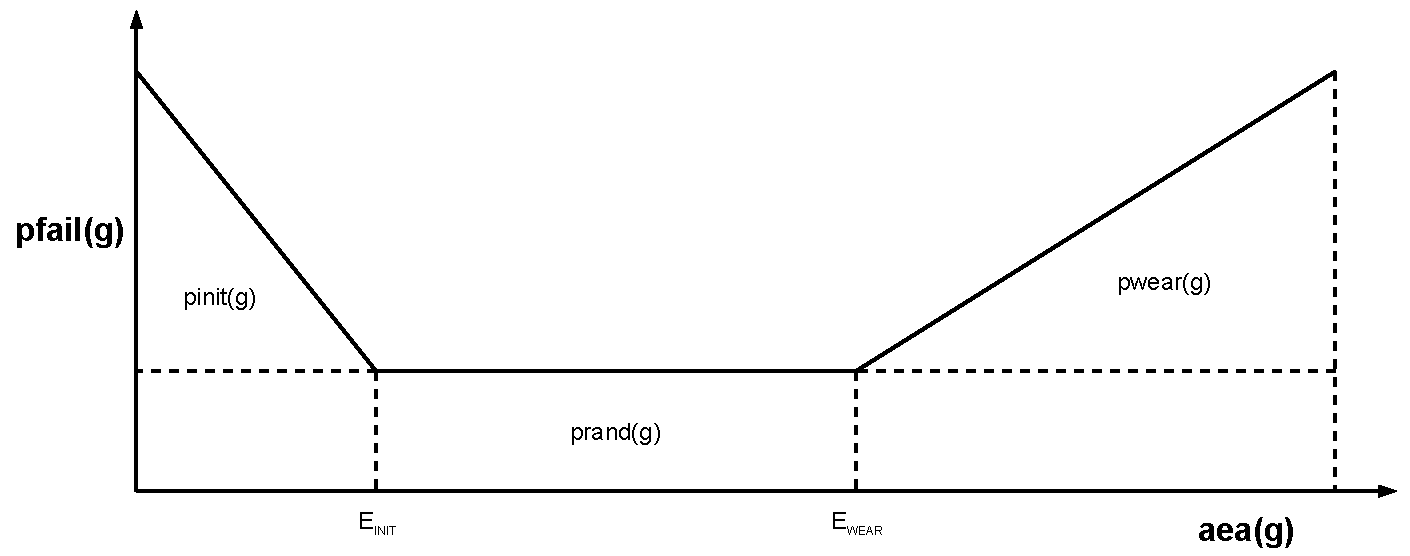
\includegraphics[width=0.7\linewidth]{node_reliability_lifespan}
	\caption[Probability of failure with lifetime energy usage for a node]{Probability of failure with lifetime energy usage for a node}
	\label{fig:node_reliability_lifespan}
\end{figure}
\begin{enumerate}
	\item $\functionProbabilityInit{}{}$, the initial failure probability, component failures early in lifespan, decreasing with time.
	\item $\functionProbabilityRand{}{}$, the random failure probability, the constant background failure rate.
	\item $\functionProbabilityWear{}{}$, the wear-out failure probability, the increasing failure rate towards the end of a nodes expected lifespan.
\end{enumerate}
For each node, we use $\functionAgentEnergyTotal{}{}$ as a proxy for time so the probability of an agent $\varAgent{}{}$ having a permanent failure increases with usage.

\definition[Probability of node failure]{
	The probability of node failure for an agent $\varAgent{}{}$ is $\functionProbabilityFail{}{}$, the combination of the probabilities of initial, random, and wear-out failures given the agents total energy usage in its lifetime $\functionAgentEnergyTotal{}{}$.
\begin{equation}
	\functionProbabilityFail{}{} = \underbrace{max(0, (1 - \functionAgentEnergyTotal{}{}/\varEnergyInit{}{})) \times \varConstantInit{}{}}_{\functionProbabilityInit{}{}} + \underbrace{\varConstantRand{}{}}_{\functionProbabilityRand{}{}} + \underbrace{max(0, ( \functionAgentEnergyTotal{}{}/\varEnergyWear{}{}))\times \varConstantWear{}{}}_{\functionProbabilityWear{}{}}
\end{equation}
	Where $\varEnergyInit{}{}{}{}$ is the energy level where initial failures are effectively zero,  and $\varEnergyWear{}{}{}{}$ where wear-out failures become a factor. $\varConstantInit{}{}$, $\varConstantRand{}{}$, and $\varConstantWear{}{}$  are constants chosen to scale the effects of initial failures and wear-out failures respectively.
}

\subsection{Coverage and resilience of routing}

\subsubsection{Coverage}

\begin{definition}[Composite task coverage]
	Given a composite task $\varCompositeTask{}{}$, and completes or partially completes this task $\varCompositeTask{}{*} \subseteq \varCompositeTask{}{}$ then the \textit{composite task coverage} of $\varCompositeTask{}{}$ is the fraction of successfully completed atomic tasks of the composite task.
	\begin{equation}
		\functionCompositeTaskCoverage{}{} = \frac{
			\funcSize{\varCompositeTask{}{*}
			}
		}{
			\funcSize{\varCompositeTask{}{}
		}
	}
	\end{equation}
\end{definition}


\subsubsection{Route adaptation}
Figure \ref{fig:wsnhierarchicalresolution} shows one of the possible modes of hierarchical networking that can be formed by the agent system through per-agent local neighbourhood learning. The initial agent passes requests through smaller and smaller neighbourhoods until the granulaity of the data meets that of the request

\begin{figure}[ht]
	\centering
	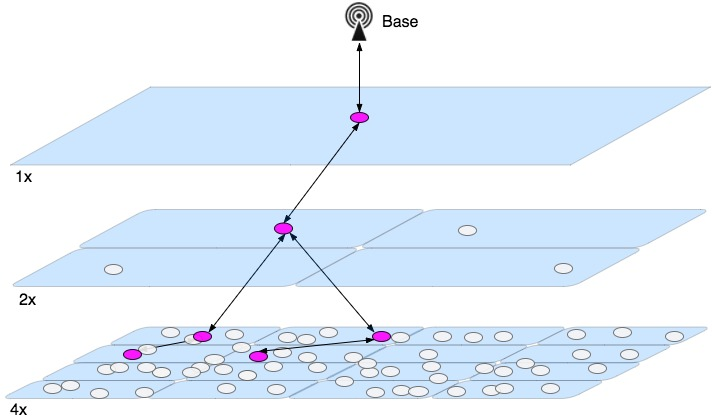
\includegraphics[width=0.5\linewidth]{WSN_hierarchical_resolution}
	\caption{Agent system hierarchical neighbourhood resolution}
	\label{fig:wsnhierarchicalresolution}
\end{figure}
In Figure \ref{fig:wsnsimulationmapfailureadaptation}, the first figure shows a set of agents aggregating data across a defined granularity geographical area using their learned neighbourhoods. In the second we see the adaptation of each agents local neighbourhood as they individually react to device failures
\begin{figure}[ht]
	\centering
	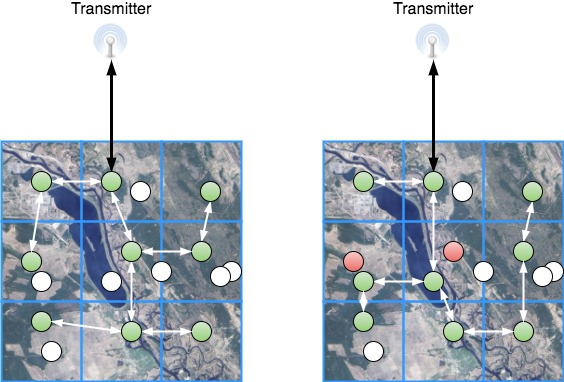
\includegraphics[width=0.5\linewidth]{WSN_simulation_map_failure_adaptation}
	\caption{WSN simulation failure adaptation}
	\label{fig:wsnsimulationmapfailureadaptation}
\end{figure}

\subsection{Defining the problem}
\todo[inline]{TODO}\subsection{Components and energy usage}

Example values in \ref{table:components_energy_usage} show the energy and time costs of varios operations given an hourly sampling period for a node.


\begin{table}
\begin{tabular}{p{0.5\textwidth}p{0.2\textwidth} p{0.2\textwidth} }
\hline
Function & power(mW) & time (s) \\
\hline
Data aquisition (DAQ) & 0.5 & 60 \\
Transmission (TX) & 7 & 0.1 \\
Broadcast (BX) & 70 & 0.1 \\
Idle wake-up-radio (WUR) & 0.07 & 3509 \\
\end{tabular}
\caption{Component types and energy usage}
\label{table:components_energy_usage}
\end{table}

\section{Problem definition}

\todo[inline]{State the optimisation problem explicitly given the system as described}
